\section{Register description}
\regover{
{\hyperref[tmr-TCCR]{TCCR}}&Timer clock source configuration register
\\
\hline
{\hyperref[tmr-TMR2-0]{TMR2\_0}}&Timer2 match register 0
\\
\hline
{\hyperref[tmr-TMR2-1]{TMR2\_1}}&Timer2 match register 1
\\
\hline
{\hyperref[tmr-TMR2-2]{TMR2\_2}}&Timer2 match register 2
\\
\hline
{\hyperref[tmr-TMR2-0]{TMR2\_0}}&Timer3 match register 0
\\
\hline
{\hyperref[tmr-TMR2-1]{TMR2\_1}}&Timer3 match register 1
\\
\hline
{\hyperref[tmr-TMR2-2]{TMR2\_2}}&Timer3 match register 2
\\
\hline
{\hyperref[tmr-TCR2]{TCR2}}&Timer2 counter register
\\
\hline
{\hyperref[tmr-TCR3]{TCR3}}&Timer3 counter register
\\
\hline
{\hyperref[tmr-TMSR2]{TMSR2}}&Timer2 match register status
\\
\hline
{\hyperref[tmr-TMSR3]{TMSR3}}&Timer3 match register status
\\
\hline
{\hyperref[tmr-TIER2]{TIER2}}&Timer2 match interrupt enable register
\\
\hline
{\hyperref[tmr-TIER3]{TIER3}}&Timer3 match interrupt enable register
\\
\hline
{\hyperref[tmr-TPLVR2]{TPLVR2}}&Timer2 pre-load value register
\\
\hline
{\hyperref[tmr-TPLVR3]{TPLVR3}}&Timer3 pre-load value register
\\
\hline
{\hyperref[tmr-TPLCR2]{TPLCR2}}&Timer2 pre-load control register
\\
\hline
{\hyperref[tmr-TPLCR3]{TPLCR3}}&Timer3 pre-load control register
\\
\hline
{\hyperref[tmr-WMER]{WMER}}&WDT reset/interrupt mode register
\\
\hline
{\hyperref[tmr-WMR]{WMR}}&WDT counter match value register
\\
\hline
{\hyperref[tmr-WVR]{WVR}}&WDT counter value register
\\
\hline
{\hyperref[tmr-WSR]{WSR}}&WDT timer reset indication register
\\
\hline
{\hyperref[tmr-TICR2]{TICR2}}&Timer2 Interrupt clear control register
\\
\hline
{\hyperref[tmr-TICR3]{TICR3}}&Timer3 Interrupt clear control register
\\
\hline
{\hyperref[tmr-WICR]{WICR}}&WDT Interrupt clear register
\\
\hline
{\hyperref[tmr-TCER]{TCER}}&Timer count enable register
\\
\hline
{\hyperref[tmr-TCMR]{TCMR}}&Timer count mode register
\\
\hline
{\hyperref[tmr-TILR2]{TILR2}}&Timer2 match interrupt mode register
\\
\hline
{\hyperref[tmr-TILR3]{TILR3}}&Timer3 match interrupt mode register
\\
\hline
{\hyperref[tmr-WCR]{WCR}}&WDT timer count reset register
\\
\hline
{\hyperref[tmr-WFAR]{WFAR}}&WDT access key1 register
\\
\hline
{\hyperref[tmr-WSAR]{WSAR}}&WDT access key2 register
\\
\hline
{\hyperref[tmr-TCVWR2]{TCVWR2}}&Timer2 capture value of counter register
\\
\hline
{\hyperref[tmr-TCVWR3]{TCVWR3}}&Timer3 capture value of counter register
\\
\hline
{\hyperref[tmr-TCVSYN2]{TCVSYN2}}&Timer2 synchronous value of counter register
\\
\hline
{\hyperref[tmr-TCVSYN3]{TCVSYN3}}&Timer3 synchronous value of counter register
\\
\hline
{\hyperref[tmr-TCDR]{TCDR}}&WDT/Timer clock division register
\\
\hline
}

\subsection{TCCR}
\label{tmr-TCCR}
Address:0x4000a500
 \begin{figure}[H]
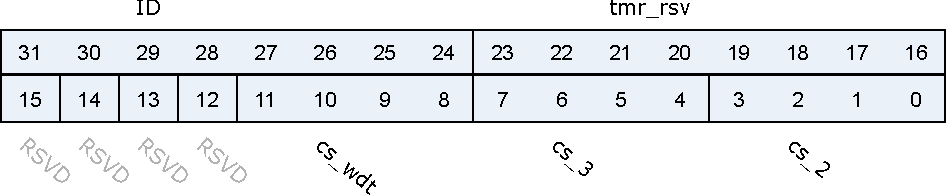
\includegraphics{tmr_TCCR.pdf}
\end{figure}

\regdes{31:10&RSVD& & & \\\hline
9:8&cs\_wdt&r/w&2'd0&Clock Source for Timer \#1/\#2/\#3/WDT \par 2'd0 - fclk \par 2'd1 - f32k\_clk \par 2'd2 - 1 kHz \par 2'd3 - PLL 32MHz
\\\hline
7&RSVD& & & \\\hline
6:5&cs\_2&r/w&2'd0&\\\hline
4&RSVD& & & \\\hline
3:2&cs\_1&r/w&2'd0&\\\hline
1:0&RSVD& & & \\\hline

}
\subsection{TMR2\_0}
\label{tmr-TMR2-0}
Address:0x4000a510
 \begin{figure}[H]
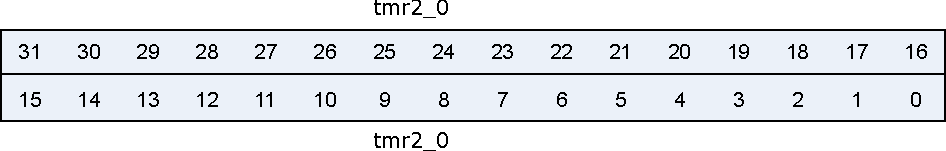
\includegraphics{tmr_TMR2_0.pdf}
\end{figure}

\regdes{31:0&tmr\_2\_0&r/w&32'hffffffff&Timer2 match register 0\\\hline

}
\subsection{TMR2\_1}
\label{tmr-TMR2-1}
Address:0x4000a514
 \begin{figure}[H]
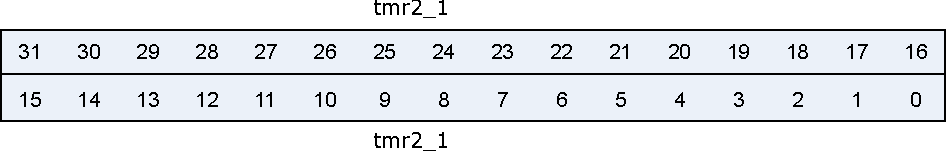
\includegraphics{tmr_TMR2_1.pdf}
\end{figure}

\regdes{31:0&tmr\_2\_1&r/w&32'hffffffff&Timer2 match register 1\\\hline

}
\subsection{TMR2\_2}
\label{tmr-TMR2-2}
Address:0x4000a518
 \begin{figure}[H]
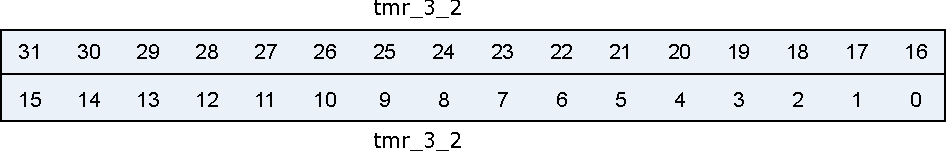
\includegraphics{tmr_TMR2_2.pdf}
\end{figure}

\regdes{31:0&tmr\_2\_2&r/w&32'hffffffff&Timer2 match register 2\\\hline

}
\subsection{TMR2\_0}
\label{tmr-TMR2-0}
Address:0x4000a51c
 \begin{figure}[H]
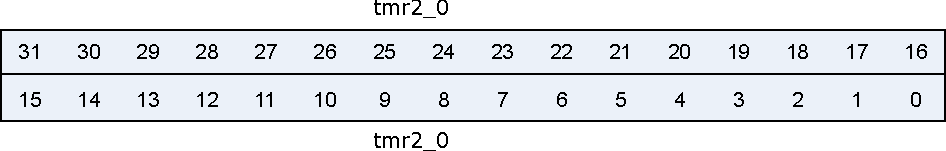
\includegraphics{tmr_TMR2_0.pdf}
\end{figure}

\regdes{31:0&tmr\_3\_0&r/w&32'hffffffff&Timer3 match register 0\\\hline

}
\subsection{TMR2\_1}
\label{tmr-TMR2-1}
Address:0x4000a520
 \begin{figure}[H]
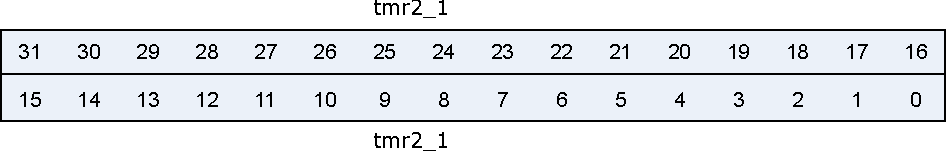
\includegraphics{tmr_TMR2_1.pdf}
\end{figure}

\regdes{31:0&tmr\_3\_1&r/w&32'hffffffff&Timer3 match register 1\\\hline

}
\subsection{TMR2\_2}
\label{tmr-TMR2-2}
Address:0x4000a524
 \begin{figure}[H]
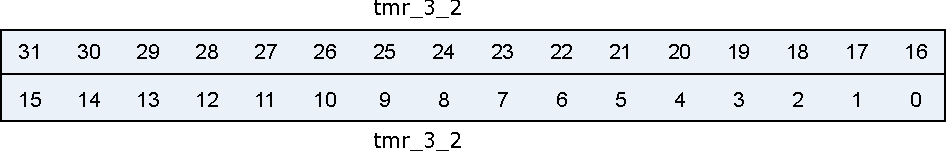
\includegraphics{tmr_TMR2_2.pdf}
\end{figure}

\regdes{31:0&tmr\_3\_2&r/w&32'hffffffff&Timer3 match register 2\\\hline

}
\subsection{TCR2}
\label{tmr-TCR2}
Address:0x4000a52c
 \begin{figure}[H]
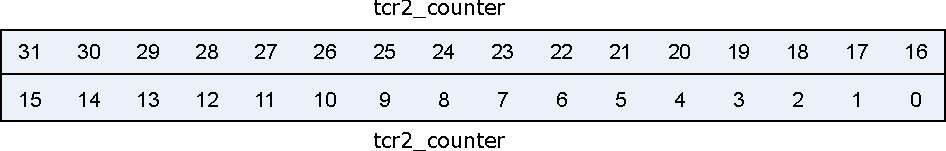
\includegraphics{tmr_TCR2.pdf}
\end{figure}

\regdes{31:0&tcr2\_counter&r&32'h0&Timer2 counter register\\\hline

}
\subsection{TCR3}
\label{tmr-TCR3}
Address:0x4000a530
 \begin{figure}[H]
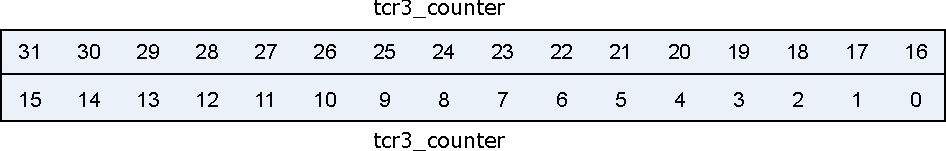
\includegraphics{tmr_TCR3.pdf}
\end{figure}

\regdes{31:0&tcr3\_counter&r&32'h0&Timer3 counter register\\\hline

}
\subsection{TMSR2}
\label{tmr-TMSR2}
Address:0x4000a538
 \begin{figure}[H]
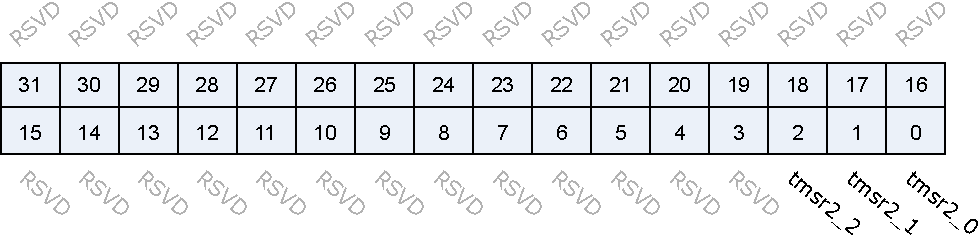
\includegraphics{tmr_TMSR2.pdf}
\end{figure}

\regdes{31:3&RSVD& & & \\\hline
2&tmsr2\_2&r&1'b0&Timer2 match register 2 status/Clear interrupt would also clear this bit\\\hline
1&tmsr2\_1&r&1'b0&Timer2 match register 1 status/Clear interrupt would also clear this bit\\\hline
0&tmsr2\_0&r&1'b0&Timer2 match register 0 status/Clear interrupt would also clear this bit\\\hline

}
\subsection{TMSR3}
\label{tmr-TMSR3}
Address:0x4000a53c
 \begin{figure}[H]
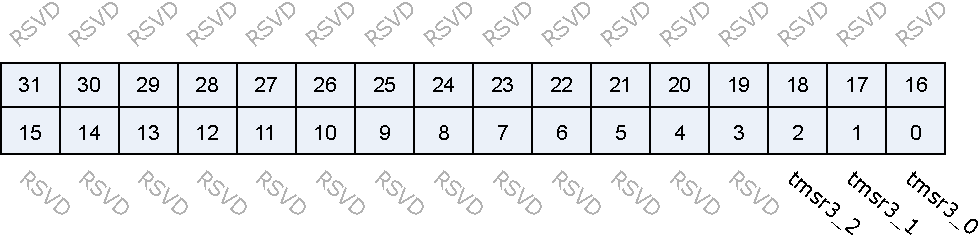
\includegraphics{tmr_TMSR3.pdf}
\end{figure}

\regdes{31:3&RSVD& & & \\\hline
2&tmsr3\_2&r&1'b0&Timer3 match register 2 status/Clear interrupt would also clear this bit\\\hline
1&tmsr3\_1&r&1'b0&Timer3 match register 1 status/Clear interrupt would also clear this bit\\\hline
0&tmsr3\_0&r&1'b0&Timer3 match register 0 status/Clear interrupt would also clear this bit\\\hline

}
\subsection{TIER2}
\label{tmr-TIER2}
Address:0x4000a544
 \begin{figure}[H]
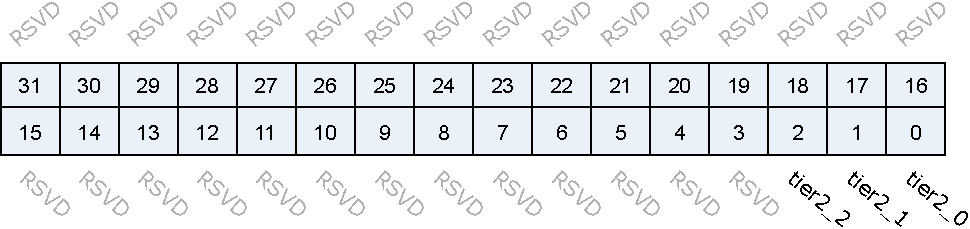
\includegraphics{tmr_TIER2.pdf}
\end{figure}

\regdes{31:3&RSVD& & & \\\hline
2&tier2\_2&r/w&1'b0&Timer2 match register 2 interrupt enable register\\\hline
1&tier2\_1&r/w&1'b0&Timer2 match register 1 interrupt enable register\\\hline
0&tier2\_0&r/w&1'b0&Timer2 match register 0 interrupt enable register\\\hline

}
\subsection{TIER3}
\label{tmr-TIER3}
Address:0x4000a548
 \begin{figure}[H]
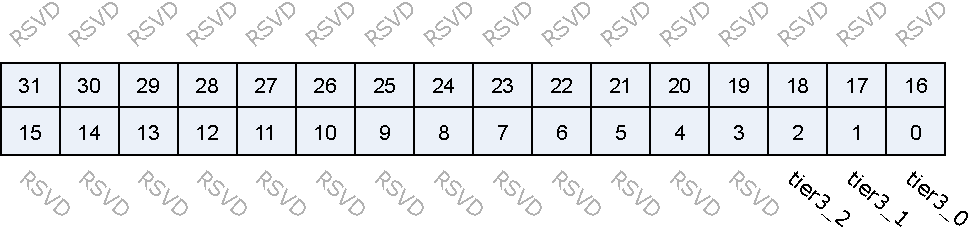
\includegraphics{tmr_TIER3.pdf}
\end{figure}

\regdes{31:3&RSVD& & & \\\hline
2&tier3\_2&r/w&1'b0&Timer3 match register 2 interrupt enable register\\\hline
1&tier3\_1&r/w&1'b0&Timer3 match register 1 interrupt enable register\\\hline
0&tier3\_0&r/w&1'b0&Timer3 match register 0 interrupt enable register\\\hline

}
\subsection{TPLVR2}
\label{tmr-TPLVR2}
Address:0x4000a550
 \begin{figure}[H]
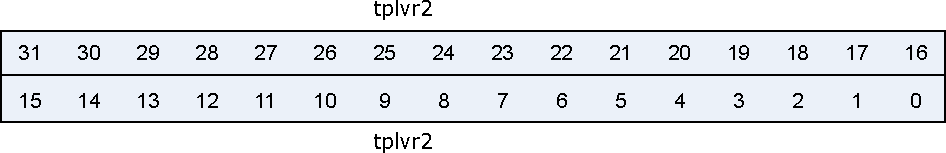
\includegraphics{tmr_TPLVR2.pdf}
\end{figure}

\regdes{31:0&tplvr2&r/w&32'h0&Timer2 pre-load value register\\\hline

}
\subsection{TPLVR3}
\label{tmr-TPLVR3}
Address:0x4000a554
 \begin{figure}[H]
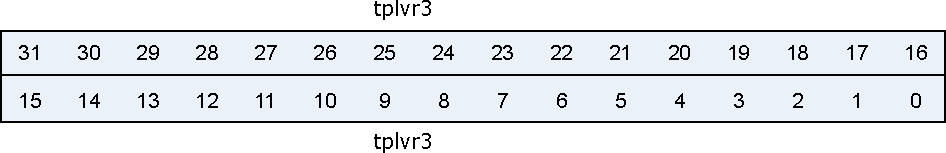
\includegraphics{tmr_TPLVR3.pdf}
\end{figure}

\regdes{31:0&tplvr3&r/w&32'h0&Timer3 pre-load value register\\\hline

}
\subsection{TPLCR2}
\label{tmr-TPLCR2}
Address:0x4000a55c
 \begin{figure}[H]
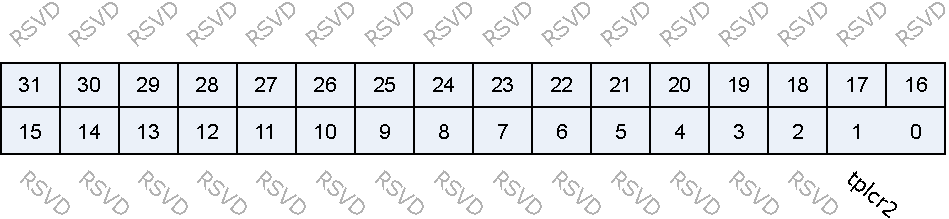
\includegraphics{tmr_TPLCR2.pdf}
\end{figure}

\regdes{31:2&RSVD& & & \\\hline
1:0&tplcr2&r/w&2'h0&Timer2 pre-load control register \par 2'd0 - No pre-load \par 2'd1 - Pre-load with match comparator 0 \par 2'd2 - Pre-load with match comparator 1 \par 2'd3 - Pre-load with match comparator 2
\\\hline

}
\subsection{TPLCR3}
\label{tmr-TPLCR3}
Address:0x4000a560
 \begin{figure}[H]
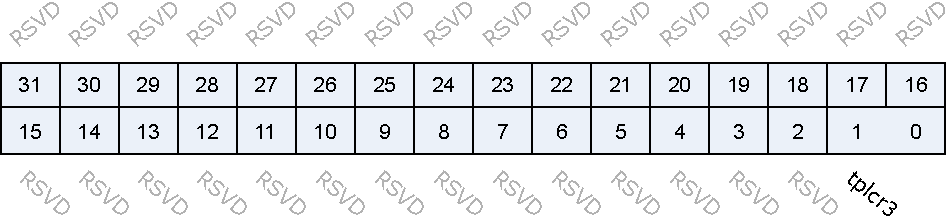
\includegraphics{tmr_TPLCR3.pdf}
\end{figure}

\regdes{31:2&RSVD& & & \\\hline
1:0&tplcr3&r/w&2'h0&Timer3 pre-load control register \par 2'd0 - No pre-load \par 2'd1 - Pre-load with match comparator 0 \par 2'd2 - Pre-load with match comparator 1 \par 2'd3 - Pre-load with match comparator 2
\\\hline

}
\subsection{WMER}
\label{tmr-WMER}
Address:0x4000a564
 \begin{figure}[H]
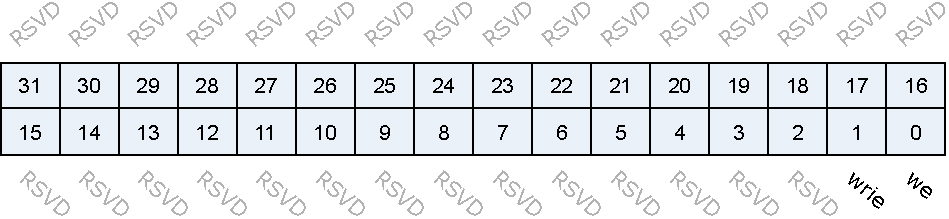
\includegraphics{tmr_WMER.pdf}
\end{figure}

\regdes{31:2&RSVD& & & \\\hline
1&wrie&r/w&1'b0&WDT reset/interrupt mode register \par 1'b0 - WDT expiration to generate interrupt \par 1'b1 - WDT expiration to generate reset source
\\\hline
0&we&r/w&1'b0&WDT enable register\\\hline

}
\subsection{WMR}
\label{tmr-WMR}
Address:0x4000a568
 \begin{figure}[H]
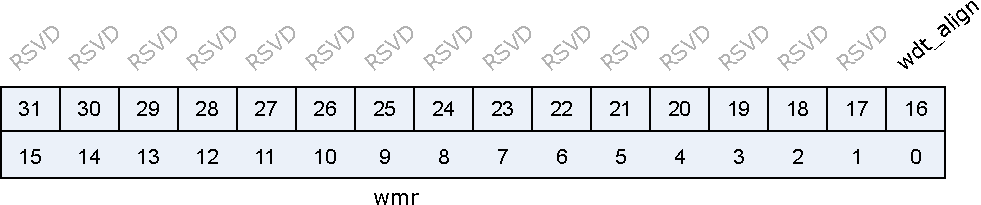
\includegraphics{tmr_WMR.pdf}
\end{figure}

\regdes{31:16&RSVD& & & \\\hline
15:0&wmr&r/w&16'hffff&WDT counter match value register\\\hline

}
\subsection{WVR}
\label{tmr-WVR}
Address:0x4000a56c
 \begin{figure}[H]
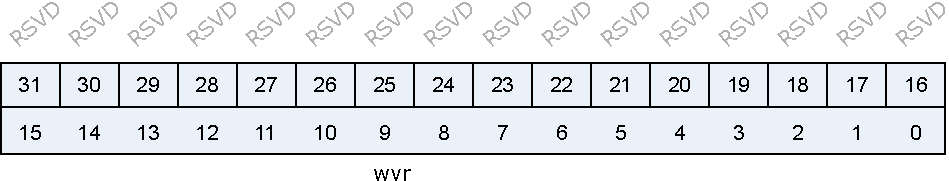
\includegraphics{tmr_WVR.pdf}
\end{figure}

\regdes{31:16&RSVD& & & \\\hline
15:0&wvr&r&16'h0&WDT counter value register\\\hline

}
\subsection{WSR}
\label{tmr-WSR}
Address:0x4000a570
 \begin{figure}[H]
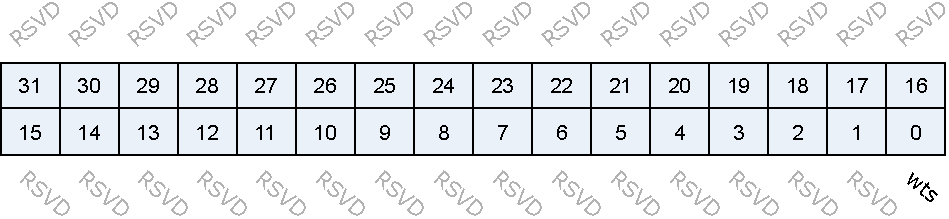
\includegraphics{tmr_WSR.pdf}
\end{figure}

\regdes{31:1&RSVD& & & \\\hline
0&wts&r/w&1'b0&WDT timer reset indication, Indicates that reset was caused by the WDT. \par (Write)1'b0 - clear the WDT reset status \par (Write)1'b1 - no affect \par (Read)1'b0 - Watchdog timer did not cause reset because this bit was cleare \par (Read)1'b1 - Watchdog timer caused reset
\\\hline

}
\subsection{TICR2}
\label{tmr-TICR2}
Address:0x4000a578
 \begin{figure}[H]
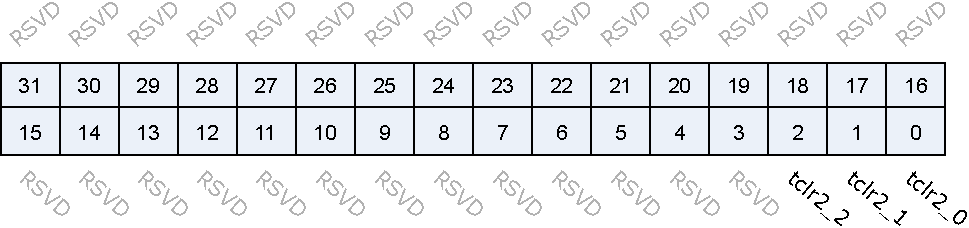
\includegraphics{tmr_TICR2.pdf}
\end{figure}

\regdes{31:3&RSVD& & & \\\hline
2&tclr2\_2&w&1'b0&Timer2 Interrupt clear for match comparator 2\\\hline
1&tclr2\_1&w&1'b0&Timer2 Interrupt clear for match comparator 1\\\hline
0&tclr2\_0&w&1'b0&Timer2 Interrupt clear for match comparator 0\\\hline

}
\subsection{TICR3}
\label{tmr-TICR3}
Address:0x4000a57c
 \begin{figure}[H]
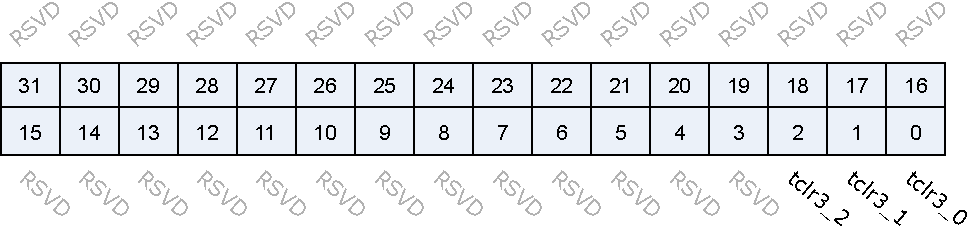
\includegraphics{tmr_TICR3.pdf}
\end{figure}

\regdes{31:3&RSVD& & & \\\hline
2&tclr3\_2&w&1'b0&Timer3 Interrupt clear for match comparator 2\\\hline
1&tclr3\_1&w&1'b0&Timer3 Interrupt clear for match comparator 1\\\hline
0&tclr3\_0&w&1'b0&Timer3 Interrupt clear for match comparator 0\\\hline

}
\subsection{WICR}
\label{tmr-WICR}
Address:0x4000a580
 \begin{figure}[H]
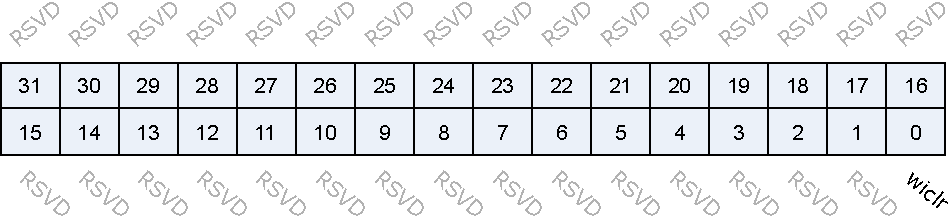
\includegraphics{tmr_WICR.pdf}
\end{figure}

\regdes{31:1&RSVD& & & \\\hline
0&wiclr&w&1'b0&WDT Interrupt clear register\\\hline

}
\subsection{TCER}
\label{tmr-TCER}
Address:0x4000a584
 \begin{figure}[H]
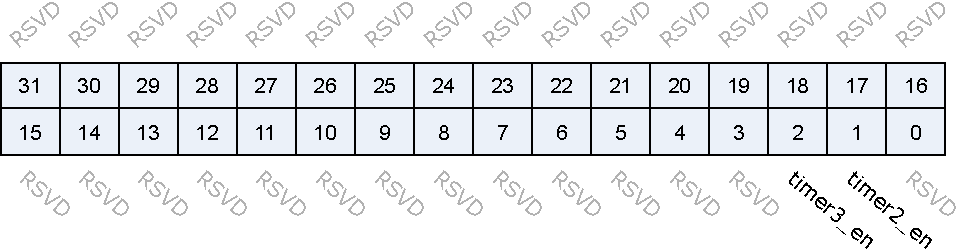
\includegraphics{tmr_TCER.pdf}
\end{figure}

\regdes{31:3&RSVD& & & \\\hline
2&timer3\_en&r/w&1'b0&Timer3 count enable\\\hline
1&timer2\_en&r/w&1'b0&Timer2 count enable\\\hline
0&RSVD& & & \\\hline

}
\subsection{TCMR}
\label{tmr-TCMR}
Address:0x4000a588
 \begin{figure}[H]
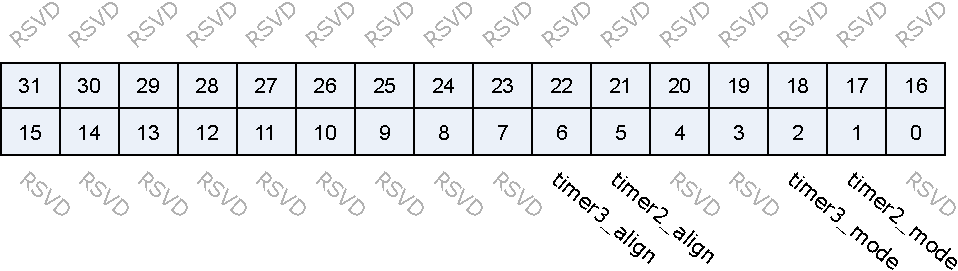
\includegraphics{tmr_TCMR.pdf}
\end{figure}

\regdes{31:3&RSVD& & & \\\hline
2&timer3\_mode&r/w&1'b0&Timer1/2/3 count mode register \par 1'b0 - pre-load mode \par 1'b1 - free run mode
\\\hline
1&timer2\_mode&r/w&1'b0&\\\hline
0&RSVD& & & \\\hline

}
\subsection{TILR2}
\label{tmr-TILR2}
Address:0x4000a590
 \begin{figure}[H]
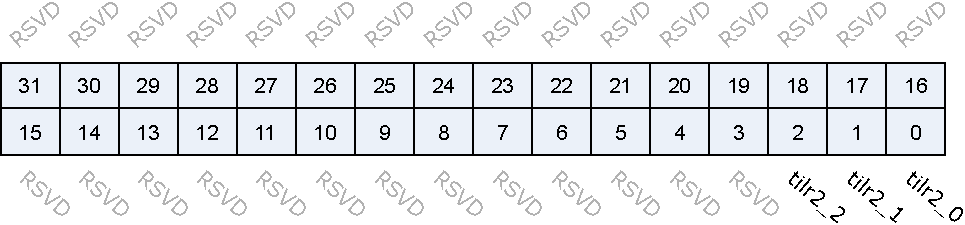
\includegraphics{tmr_TILR2.pdf}
\end{figure}

\regdes{31:3&RSVD& & & \\\hline
2&tilr2\_2&r/w&1'b0&Timer2 match 0/1/2 interrupt mode register \par 1'b0 - level interrupt \par 1'b1 - pulse interrupt
\\\hline
1&tilr2\_1&r/w&1'b0&\\\hline
0&tilr2\_0&r/w&1'b0&\\\hline

}
\subsection{TILR3}
\label{tmr-TILR3}
Address:0x4000a594
 \begin{figure}[H]
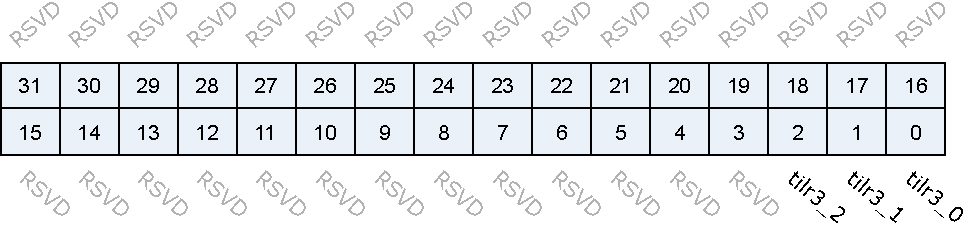
\includegraphics{tmr_TILR3.pdf}
\end{figure}

\regdes{31:3&RSVD& & & \\\hline
2&tilr3\_2&r/w&1'b0&Timer3 match 0/1/2 interrupt mode register \par 1'b0 - level interrupt \par 1'b1 - pulse interrupt
\\\hline
1&tilr3\_1&r/w&1'b0&\\\hline
0&tilr3\_0&r/w&1'b0&\\\hline

}
\subsection{WCR}
\label{tmr-WCR}
Address:0x4000a598
 \begin{figure}[H]
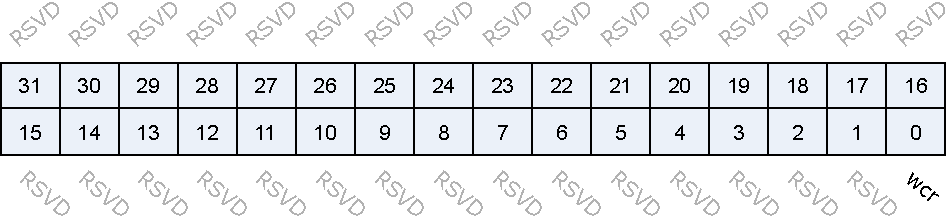
\includegraphics{tmr_WCR.pdf}
\end{figure}

\regdes{31:1&RSVD& & & \\\hline
0&wcr&w&1'b0&WDT timer count reset register\\\hline

}
\subsection{WFAR}
\label{tmr-WFAR}
Address:0x4000a59c
 \begin{figure}[H]
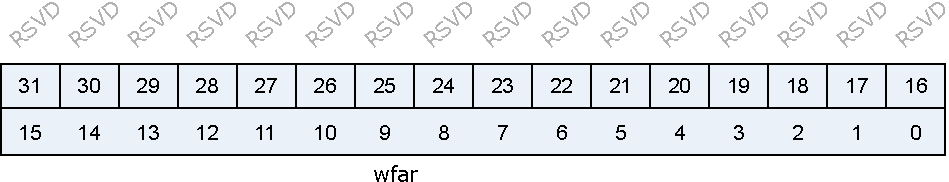
\includegraphics{tmr_WFAR.pdf}
\end{figure}

\regdes{31:16&RSVD& & & \\\hline
15:0&wfar&w&16'b0&WDT access key1 - 16'hBABA\\\hline

}
\subsection{WSAR}
\label{tmr-WSAR}
Address:0x4000a5a0
 \begin{figure}[H]
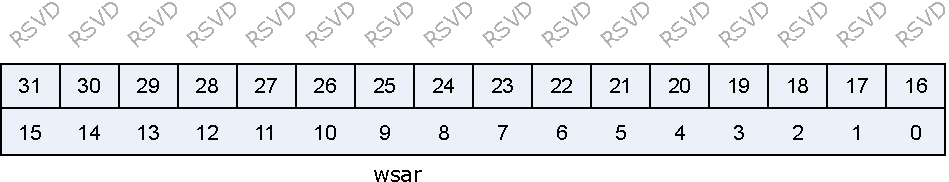
\includegraphics{tmr_WSAR.pdf}
\end{figure}

\regdes{31:16&RSVD& & & \\\hline
15:0&wsar&w&16'b0&WDT access key2 - 16'hEB10\\\hline

}
\subsection{TCVWR2}
\label{tmr-TCVWR2}
Address:0x4000a5a8
 \begin{figure}[H]
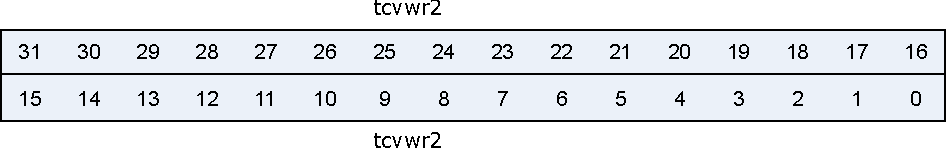
\includegraphics{tmr_TCVWR2.pdf}
\end{figure}

\regdes{31:0&tcvwr2&r&32'h0&Timer2 capture value of counter\\\hline

}
\subsection{TCVWR3}
\label{tmr-TCVWR3}
Address:0x4000a5ac
 \begin{figure}[H]
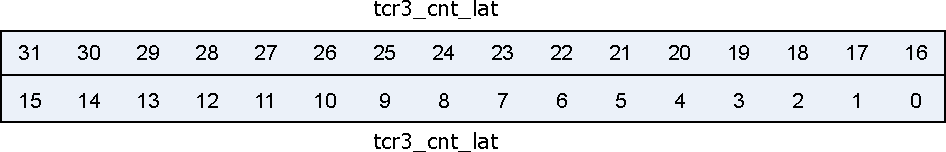
\includegraphics{tmr_TCVWR3.pdf}
\end{figure}

\regdes{31:0&tcvwr3&r&32'h0&Timer3 capture value of counter\\\hline

}
\subsection{TCVSYN2}
\label{tmr-TCVSYN2}
Address:0x4000a5b4
 \begin{figure}[H]
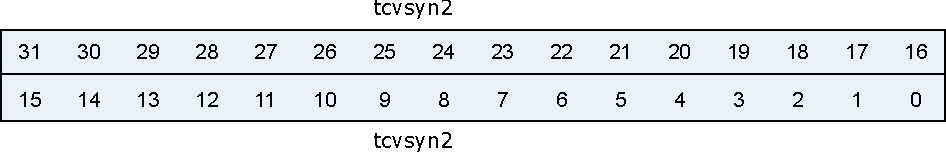
\includegraphics{tmr_TCVSYN2.pdf}
\end{figure}

\regdes{31:0&tcvsyn2&r&32'h0&Timer2 synchronous value of counter\\\hline

}
\subsection{TCVSYN3}
\label{tmr-TCVSYN3}
Address:0x4000a5b8
 \begin{figure}[H]
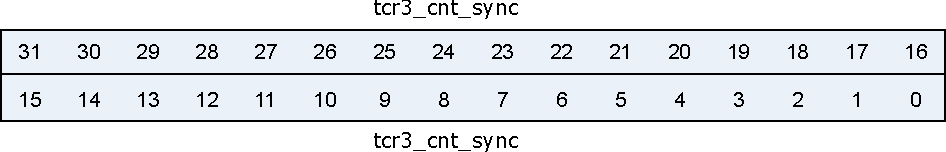
\includegraphics{tmr_TCVSYN3.pdf}
\end{figure}

\regdes{31:0&tcvsyn3&r&32'h0&Timer3 synchronous value of counter\\\hline

}
\subsection{TCDR}
\label{tmr-TCDR}
Address:0x4000a5bc
 \begin{figure}[H]
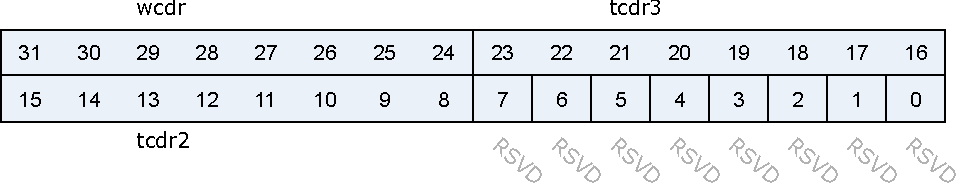
\includegraphics{tmr_TCDR.pdf}
\end{figure}

\regdes{31:24&wcdr&r/w&8'h0&WDT clock division value register\\\hline
23:16&tcdr3&r/w&8'h0&Timer3 clock division value register\\\hline
15:8&tcdr2&r/w&8'h0&Timer2 clock division value register\\\hline
7:0&RSVD& & & \\\hline

}
